\chapter{Background and Technical Foundation}

\section{Introduction}

This chapter establishes the technical foundation necessary for understanding the GitOps versus Traditional CI/CD comparative analysis implemented through the TechMart platform. The chapter examines deployment methodology evolution, key technical concepts, and research context essential for comprehending the empirical investigation presented in subsequent chapters.

The foundation encompasses deployment methodology principles, technical implementation rationale, and research gaps that motivate this empirical study. Understanding these elements is crucial for interpreting the research methodology, implementation choices, and analytical frameworks employed in this investigation.

\section{Deployment Methodology Evolution}

\subsection{Traditional CI/CD Principles and Current Limitations}

Continuous Integration and Continuous Deployment emerged to address manual, error-prone deployment processes through automated build, test, and deployment workflows \cite{fowler2013continuous, kim2016devops}. Traditional CI/CD methodologies employ imperative scripting approaches that explicitly define deployment steps, resource allocation procedures, and environment configuration management through centralized pipeline systems.

Traditional CI/CD has demonstrated significant value in improving deployment frequency and reducing manual errors compared to manual processes. However, contemporary implementations face mounting challenges as software systems become increasingly complex:

\begin{itemize}
\item \textbf{Manual Approval Bottlenecks:} Human approval gates introduce delays ranging from minutes to hours, creating deployment bottlenecks that impact development velocity
\item \textbf{Environment Configuration Drift:} Multi-environment consistency becomes difficult as configuration variations proliferate, leading to deployment failures and debugging complexity
\item \textbf{Complex Rollback Procedures:} Manual intervention required for rollbacks, particularly with database changes or multi-service deployments, increasing recovery time during incidents
\item \textbf{Pipeline Maintenance Overhead:} Explicit pipeline definition required for each service, leading to configuration duplication and maintenance complexity
\end{itemize}

\subsection{GitOps Emergence and Core Concepts}

GitOps represents a paradigmatic shift toward declarative deployment methodologies that leverage Git repositories as the single source of truth for both application code and infrastructure configuration \cite{weaveworks2017gitops, beetz2021gitops}. This approach transforms deployment from imperative command execution to desired state convergence, where automated controllers continuously monitor Git repositories and ensure deployed environments match declared specifications.

The declarative nature of GitOps eliminates explicit deployment scripting by defining desired system state through configuration files. GitOps controllers automatically detect differences between declared and actual system state, implementing necessary changes to achieve convergence without human intervention.

Key GitOps advantages include:

\begin{itemize}
\item \textbf{Complete Automation:} Elimination of manual approval gates through Git-based approval mechanisms
\item \textbf{Self-Healing Capabilities:} Automatic drift detection and correction without human intervention
\item \textbf{Simplified Rollbacks:} Instant rollback through Git revert operations
\item \textbf{Enhanced Security:} Git-based access control and comprehensive audit trails through commit history
\item \textbf{Developer-Friendly Workflows:} Natural integration with existing Git-based development processes
\end{itemize}

\subsection{Declarative vs Imperative Deployment Approaches}

The distinction between declarative and imperative approaches represents a fundamental architectural difference impacting system reliability and operational complexity:

\begin{table}[h]
\centering
\caption{Declarative vs Imperative Deployment Comparison}
\label{tab:declarative_imperative_comparison}
\renewcommand{\arraystretch}{1.4}
\scriptsize
\begin{tabular}{|p{2.5cm}|p{4.5cm}|p{4.5cm}|}
\hline
\textbf{Aspect} & \textbf{Traditional CI/CD} & \textbf{GitOps} \\
\hline
\textbf{Deployment Model} & Explicit step execution & Desired state convergence \\
\hline
\textbf{Human Intervention} & Manual approval gates & Git-based approval only \\
\hline
\textbf{Configuration Drift} & Manual detection/correction & Automatic drift correction \\
\hline
\textbf{Rollback} & Manual procedures & Git revert operations \\
\hline
\textbf{Audit Trail} & Pipeline logs & Complete Git history \\
\hline
\textbf{Learning Curve} & Familiar to ops teams & Requires GitOps expertise \\
\hline
\end{tabular}
\end{table}

To further illustrate the differences, Figure~\ref{fig:gitops-vs-traditional-cicd} provides a visual comparison of the workflows for Traditional CI/CD and GitOps, highlighting the procedural steps and automation mechanisms.

\begin{figure}[h]
\centering
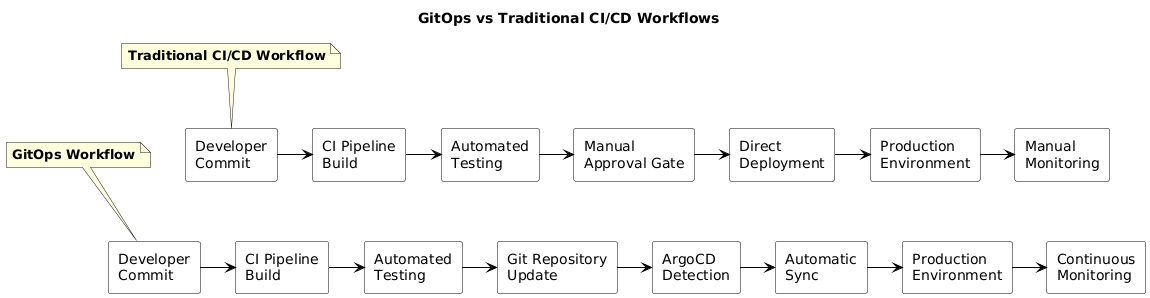
\includegraphics[width=1.0\textwidth, height=1.8\textheight, keepaspectratio]{figures/GitOp-vs-Traditional-CICD-Workflow-Comparison.png}
\caption{GitOps vs Traditional CI/CD Workflow Comparison}
\label{fig:gitops-vs-traditional-cicd}
\end{figure}

Despite theoretical advantages, fundamental questions about GitOps practical performance characteristics remain inadequately addressed. Current literature predominantly focuses on conceptual benefits without comprehensive empirical validation against Traditional CI/CD methodologies, creating uncertainty around adoption strategies and implementation decisions.

\subsection{ArgoCD and GitOps Controller Implementation}

ArgoCD represents the leading GitOps controller implementation, providing comprehensive automation for Kubernetes-based application deployment. ArgoCD continuously monitors Git repositories for configuration changes and automatically synchronizes deployed applications through sophisticated reconciliation algorithms.

ArgoCD employs a declarative application model where applications are defined through Custom Resource Definitions (CRDs) specifying Git repository locations, target namespaces, and synchronization policies. Advanced features include multi-cluster management, automated rollback procedures, and comprehensive monitoring dashboards supporting multiple configuration management tools including Helm, Kustomize, and plain Kubernetes manifests.

\section{Technical Implementation Foundation}

\subsection{Containerization and Orchestration Strategy}

Container technology provides the foundation for consistent application deployment across diverse environments. Docker containerization encapsulates applications with complete runtime dependencies, eliminating environment-specific configuration issues while enabling consistent behavior across development, testing, and production environments.

Kubernetes serves as the orchestration platform for GitOps services, providing declarative management capabilities where users specify desired application state through YAML manifests. The master-worker node architecture enables scalable container orchestration while maintaining high availability through component redundancy.

\textbf{Technology Selection Rationale:}
\begin{itemize}
\item \textbf{Docker:} Industry-standard containerization enabling consistent deployment patterns
\item \textbf{Kubernetes (GKE):} Required for GitOps methodology demonstration with ArgoCD integration
\item \textbf{Heroku Container Stack:} Platform-as-a-Service optimization for Traditional CI/CD comparison
\end{itemize}

\subsection{Multi-Cloud Strategy and Platform Selection}

Multi-cloud architecture enables strategic service placement across different providers to optimize cost, performance, and methodology demonstration. This approach leverages provider-specific capabilities while avoiding vendor lock-in and enabling realistic operational complexity for methodology evaluation.

\textbf{Platform Distribution Strategy:}
\begin{itemize}
\item \textbf{Google Kubernetes Engine:} GitOps services (User + Order) requiring sophisticated orchestration
\item \textbf{Heroku Platform-as-a-Service:} Traditional CI/CD services (Product + Cart) optimizing for simplicity
\item \textbf{Vercel:} Frontend deployment with Git integration and global CDN
\item \textbf{Supporting Services:} Database and monitoring distributed across optimal providers
\end{itemize}

Figure \ref{fig:multi-cloud-architecture} presents the comprehensive multi-cloud infrastructure architecture that enables this research, illustrating the strategic distribution of services across different cloud providers and the integration patterns between GitOps and Traditional CI/CD deployment methodologies.

\begin{figure}[H]
\centering
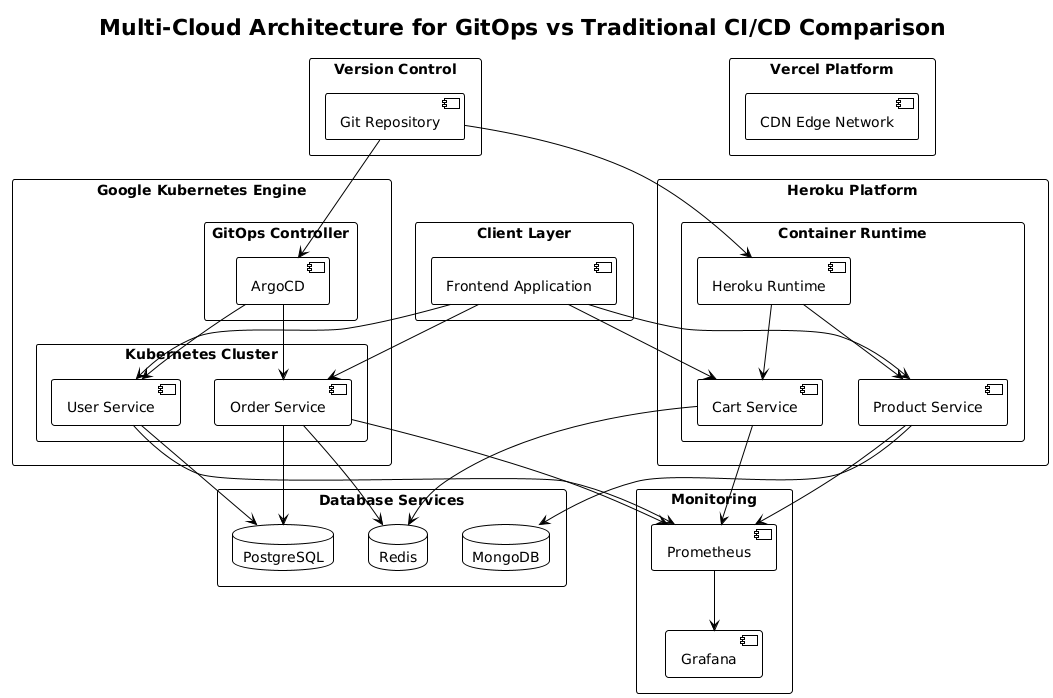
\includegraphics[width=1.0\textwidth]{figures/Multi-Cloud-Architecture-Diagram.png}
\caption{Multi-Cloud Architecture for GitOps vs Traditional CI/CD Implementation}
\label{fig:multi-cloud-architecture}
\end{figure}


The multi-cloud approach creates realistic enterprise deployment complexity while enabling controlled methodology comparison. Platform abstraction through containers enables consistent application deployment while preserving access to provider-specific optimization capabilities.

\subsection{Technology Stack Rationale for Research Design}

Technology diversity enables evaluation of methodology performance across various programming languages and frameworks while maintaining architectural coherence. The technology selection ensures fair methodology comparison by accounting for different complexity levels and performance characteristics.

\textbf{Service Technology Distribution:}

\begin{table}[h]
\centering
\caption{Technology Stack Distribution for Methodology Comparison}
\label{tab:tech_stack_distribution}
\renewcommand{\arraystretch}{1.2}
\small
\begin{tabular}{|p{2.3cm}|p{4.2cm}|p{2.4cm}|p{3.5cm}|}
\hline
\textbf{Service} & \textbf{Technology Stack} & \textbf{Methodology} & \textbf{Rationale} \\
\hline
User Service & Python FastAPI + PostgreSQL & GitOps & Authentication complexity \\
\hline
Order Service & Python FastAPI + PostgreSQL + Redis & GitOps & Multi-database integration \\
\hline
Product Service & Node.js Express + MongoDB & Traditional CI/CD & Platform optimization \\
\hline
Cart Service & Java Spring Boot + Redis & Traditional CI/CD & Enterprise framework \\
\hline
\end{tabular}
\end{table}

\textbf{Database Technology Selection:}
\begin{itemize}
\item \textbf{PostgreSQL (Neon):} Transactional data requiring ACID compliance
\item \textbf{MongoDB (Atlas):} Flexible catalog data with document structure
\item \textbf{Redis (Upstash):} High-performance session management and caching
\end{itemize}

This polyglot persistence approach demonstrates realistic enterprise complexity while enabling methodology evaluation across different data management patterns.

\section{Research Context and Literature Analysis}

\subsection{Performance Evaluation Methodologies}

Software engineering metrics provide quantitative measures enabling evidence-based decision making. Key performance indicators including response time, throughput, error rates, and resource utilization offer comprehensive system health visibility essential for methodology comparison.

\textbf{Critical Evaluation Challenges:}
\begin{itemize}
\item \textbf{Service Complexity Variations:} Different technology stacks and architectural patterns affect performance independent of deployment methodology
\item \textbf{Environment Heterogeneity:} Laboratory conditions fail to capture production complexity and resource constraints
\item \textbf{Statistical Rigor:} Lack of standardized comparison frameworks preventing meaningful cross-study analysis
\end{itemize}

Statistical analysis methodologies including hypothesis testing, confidence intervals, and effect size calculations ensure research findings are statistically sound and reproducible. Experimental design principles including controlled variables, randomization, and replication enable valid comparisons while minimizing bias and confounding factors.

\subsection{Complexity Normalization Requirements}

Fair methodology comparison requires accounting for inherent complexity factors that influence performance independent of deployment approach. Service complexity metrics including codebase size, dependency count, resource requirements, and architectural patterns provide quantitative measures enabling complexity-adjusted performance comparisons.

This research develops a novel complexity normalization framework that enables fair comparison across heterogeneous service architectures by accounting for:
\begin{itemize}
\item \textbf{Codebase Complexity:} Lines of code, structural complexity, and maintainability metrics
\item \textbf{Build Complexity:} Dependency management, compilation requirements, and pipeline sophistication
\item \textbf{Resource Intensity:} CPU, memory, and storage requirements
\item \textbf{Technology Stack Characteristics:} Framework complexity and platform optimization
\item \textbf{External Dependencies:} Service integration and operational requirements
\end{itemize}

\subsection{Related Work and Literature Review}

\subsubsection{Existing CI/CD Methodology Comparisons}

Current literature on CI/CD methodology comparison focuses predominantly on theoretical advantages and case study analysis rather than comprehensive empirical evaluation using production systems. Most studies examine GitOps and Traditional CI/CD approaches in isolation without direct performance comparison under controlled conditions.

Academic research emphasizes conceptual frameworks and best practices rather than quantitative performance analysis accounting for complexity variations and technology stack differences. This theoretical focus limits practical applicability for organizations making methodology selection decisions.

Industry studies often lack statistical rigor and reproducible methodologies while focusing on specific technology combinations that may not generalize to diverse application portfolios. Vendor-sponsored research introduces potential bias affecting credibility and objectivity of findings.

\subsubsection{GitOps Research and Industry Studies}

GitOps research has primarily focused on conceptual frameworks, implementation patterns, and case studies demonstrating successful adoptions rather than rigorous performance evaluation and comparative analysis. Academic contributions emphasize security benefits, audit capabilities, and operational simplification without quantitative validation.

Industry adoption studies typically present success stories and implementation guidance without comprehensive performance data or comparison with alternative approaches. These studies often lack statistical validation and reproducible methodologies that would enable independent verification of claims.

Tool-specific research focusing on ArgoCD, Flux, and other GitOps controllers provides implementation guidance and feature comparisons but lacks broader methodology evaluation accounting for organizational context and application characteristics.

\subsubsection{Multi-Cloud Deployment Research}

Multi-cloud research primarily examines strategy, architecture patterns, and tool evaluation rather than empirical performance analysis of deployment methodologies across different cloud providers. Most studies focus on vendor selection criteria and integration challenges rather than methodology effectiveness.

Cost optimization and performance studies typically analyze individual cloud providers or specific services rather than comprehensive methodology evaluation across multi-cloud environments. This limitation prevents understanding of methodology performance variations across different infrastructure platforms.

\subsection{Identified Research Gaps}

The analysis reveals significant gaps in current research:

\begin{itemize}
\item \textbf{Absence of Empirical Comparison:} No comprehensive production-grade comparison between GitOps and Traditional CI/CD with statistical validation
\item \textbf{Lack of Complexity Normalization:} Current studies fail to account for service complexity variations that can bias methodology evaluation
\item \textbf{Missing Hybrid Architecture Validation:} Limited research on methodology coexistence and integration patterns despite practical importance for gradual adoption
\item \textbf{Insufficient Performance Attribution:} Poor understanding of methodology-specific characteristics versus technology stack influences
\item \textbf{Lack of Optimization Frameworks:} Absence of evidence-based guidance for methodology selection and performance improvement
\end{itemize}

These gaps necessitate empirical research using production systems with complexity normalization and statistical validation to provide evidence-based insights for enterprise methodology selection decisions.

\section{Monitoring and Research Infrastructure}

Modern observability requires comprehensive metrics collection, visualization, and alerting capabilities supporting both operational monitoring and research data collection. The monitoring infrastructure must handle high-volume data streams while providing real-time analysis and historical retention for statistical validation.

\textbf{Monitoring Strategy:}
\begin{itemize}
\item \textbf{Prometheus:} Time-series metrics collection with powerful query language (PromQL) for analysis
\item \textbf{Grafana:} Comprehensive visualization and dashboard capabilities with multiple data source support
\item \textbf{GitHub Actions Integration:} Automated metrics collection during pipeline execution
\item \textbf{Application Performance Monitoring:} Distributed tracing and performance analysis across services
\end{itemize}

The monitoring approach enables both operational oversight and research data collection essential for empirical methodology validation with statistical rigor.

\section{Conclusion}

This chapter establishes the comprehensive technical foundation necessary for understanding the GitOps versus Traditional CI/CD comparative analysis. The examination of deployment methodology evolution, technical implementation rationale, and research context provides essential background for evaluating the empirical findings presented in subsequent chapters.

The identified research gaps highlight the significance of this study's contribution while the technical foundation demonstrates the sophistication required for valid comparative analysis. The progression from Traditional CI/CD limitations through GitOps innovations, implementation technology selection, and research methodology context enables detailed examination of system design, implementation, and empirical results that follow.

The literature analysis confirms the absence of comprehensive empirical comparison between methodologies with complexity normalization and statistical validation, establishing the critical need for this research to provide evidence-based insights for enterprise methodology selection decisions.